\documentclass[11pt, oneside]{article}   	% use "amsart" instead of "article" for AMSLaTeX format
\usepackage[margin = 1in]{geometry}                		% See geometry.pdf to learn the layout options. There are lots.
\geometry{letterpaper}                   		% ... or a4paper or a5paper or ... 
%\geometry{landscape}                		% Activate for rotated page geometry
%\usepackage[parfill]{parskip}    		% Activate to begin paragraphs with an empty line rather than an indent
\usepackage{graphicx}				% Use pdf, png, jpg, or eps§ with pdflatex; use eps in DVI mode
								% TeX will automatically convert eps --> pdf in pdflatex		
\usepackage{amssymb}
\usepackage{amsmath}
\usepackage[shortlabels]{enumitem}
\usepackage{float}
\usepackage{tikz-cd}
\usepackage{subcaption}
\usepackage{slashed}

\usepackage{amsthm}
\theoremstyle{definition}
\newtheorem{definition}{Definition}[section]
\newtheorem{theorem}{Theorem}[section]
\newtheorem{corollary}{Corollary}[theorem]
\newtheorem{lemma}[theorem]{Lemma}

\newcommand{\N}{\mathbb{N}}
\newcommand{\R}{\mathbb{R}}
\newcommand{\Z}{\mathbb{Z}}
\newcommand{\Q}{\mathbb{Q}}

\usepackage{simpler-wick}
\usepackage[compat=1.0.0]{tikz-feynman}   %note you need to compile this in LuaLaTeX for diagrams to render correctly

% make arrow superscripts
\DeclareFontFamily{OMS}{oasy}{\skewchar\font48 }
\DeclareFontShape{OMS}{oasy}{m}{n}{%
         <-5.5> oasy5     <5.5-6.5> oasy6
      <6.5-7.5> oasy7     <7.5-8.5> oasy8
      <8.5-9.5> oasy9     <9.5->  oasy10
      }{}
\DeclareFontShape{OMS}{oasy}{b}{n}{%
       <-6> oabsy5
      <6-8> oabsy7
      <8->  oabsy10
      }{}
\DeclareSymbolFont{oasy}{OMS}{oasy}{m}{n}
\SetSymbolFont{oasy}{bold}{OMS}{oasy}{b}{n}

\DeclareMathSymbol{\smallleftarrow}     {\mathrel}{oasy}{"20}
\DeclareMathSymbol{\smallrightarrow}    {\mathrel}{oasy}{"21}
\DeclareMathSymbol{\smallleftrightarrow}{\mathrel}{oasy}{"24}
%\newcommand{\cev}[1]{\reflectbox{\ensuremath{\vec{\reflectbox{\ensuremath{#1}}}}}}
\newcommand{\vecc}[1]{\overset{\scriptscriptstyle\smallrightarrow}{#1}}
\newcommand{\cev}[1]{\overset{\scriptscriptstyle\smallleftarrow}{#1}}
\newcommand{\cevvec}[1]{\overset{\scriptscriptstyle\smallleftrightarrow}{#1}}

\newcommand{\dbar}{d\hspace*{-0.08em}\bar{}\hspace*{0.1em}}

%SetFonts

%SetFonts


\title{The Lorentz and Poincar\'{e} Groups}
\author{Patrick Oare}
\date{}							% Activate to display a given date or no date

\begin{document}
\maketitle
\section{The Lorentz Group and Algebra}

Let $g_{\mu\nu} := diag(1, -1, -1, -1)$ be the standard Minkowski metric. The \textbf{Lorentz group}, denoted $SO(1, 3)$, is the 
subgroup of $M_{4\times 4}(\mathbb R)$ which leaves $g$ invariant under conjugation, i.e. a 4 by 4 matrix $\Lambda$ is in 
$SO(1, 3)$ iff:
\begin{equation}
	\Lambda^T g\Lambda = g
\end{equation}

As you know from Special Relativity, flat spacetime has a Minkowski metric and elements of the Lorentz group boost states 
into different frames. As a topological space, the Lorentz group is disconnected: it has four connected components, which 
correspond to where the symmetries of \textbf{parity}, $P = diag(1, -1, -1, -1)$, and \textbf{time reversal}, $T = diag(-1, 1, 1, 1)$ 
lie. We call a Lorentz transformation $\Lambda\in SO(1, 3)$ \textbf{proper} if $det(\Lambda) = 1$ and \textbf{orthochronous} if 
$\Lambda^0_0 > 1$, and we can split $SO(1, 3)$ into its connected components based on where these symmetries lie, as 
depicted in Figure~\ref{fig:lorentz}.

\begin{figure}[H]
	\centering
	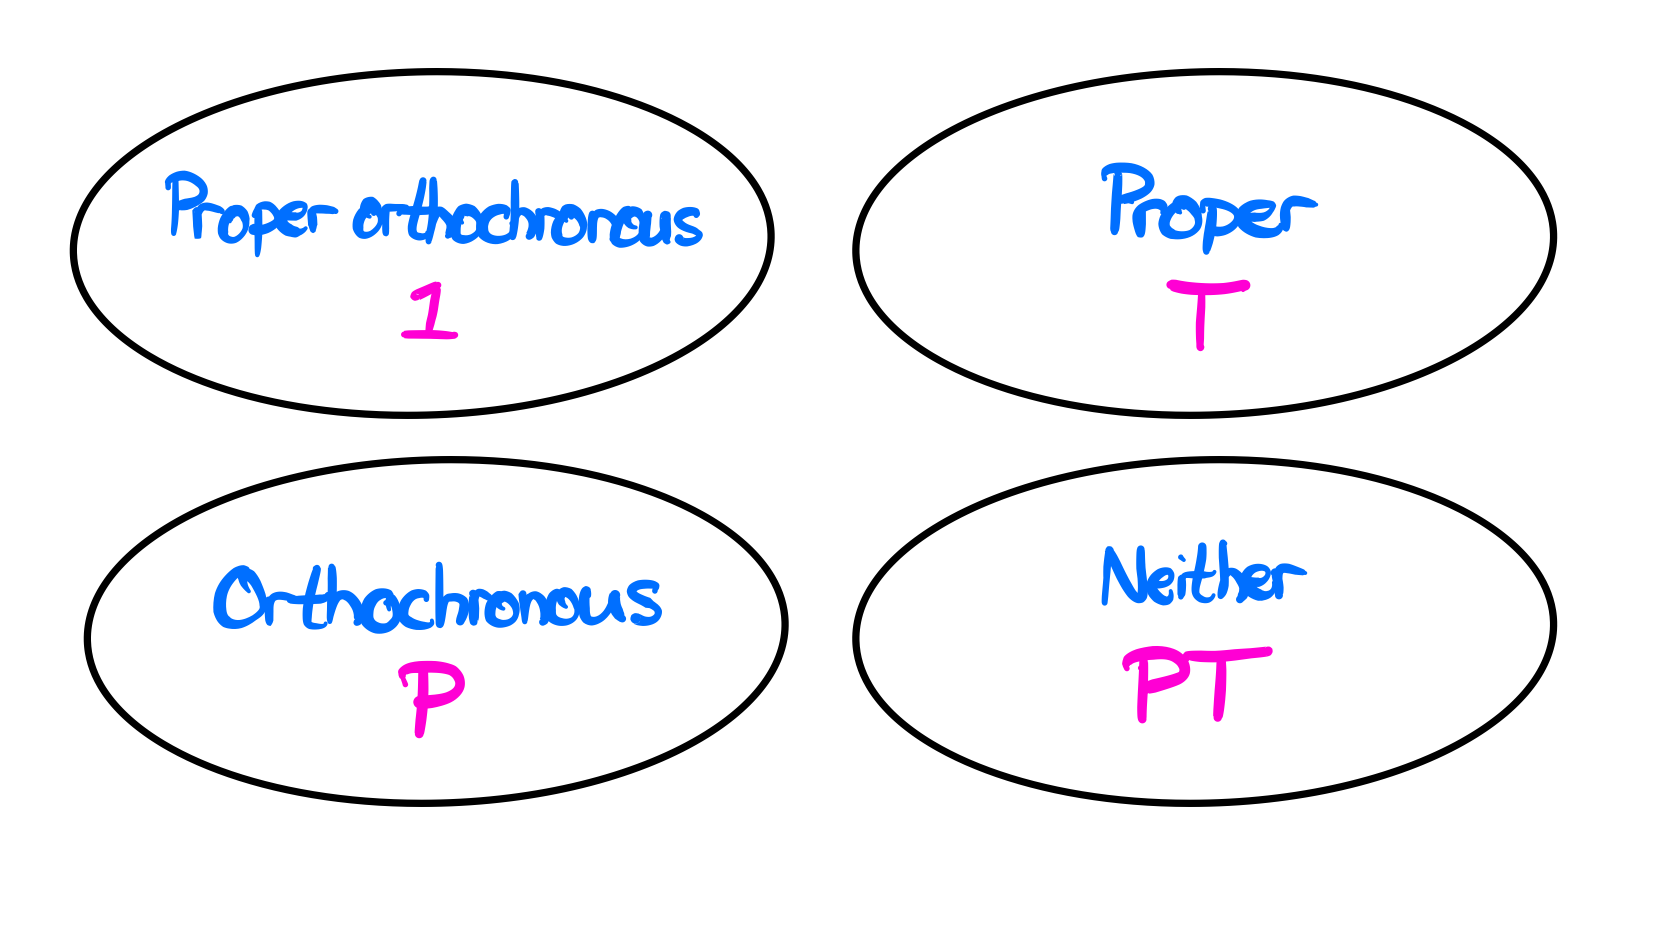
\includegraphics[width = 0.6\textwidth]{lorentz_group}
	\caption{The four connected components of the Lorentz group. The proper orthochronous component is in the neighborhood 
	of $1$, and thus the only elements that can be generated as exponentials of the Lie algebra lie in this component. Each component 
	contains exactly one of $P^a T^b$, where $a, b\in\{0, 1\}$.}~
	\label{fig:lorentz}
\end{figure}

When we study the Lie algebra $\mathfrak{so}(1, 3)$, we are only generating the proper orthochronous subset of the Lorentz group $SO(1, 
3)^+$. However, it is still very helpful to understand the structure of this subset of $SO(1, 3)$, as any arbitrary Lorentz transformation is a 
product $(\rm{proper orthochronous})\times P^a \times T^b$ for $a, b\in \{0, 1\}$. The algebra \textbf{$\mathfrak{so}(1, 3)$ has 6 generators}, 
which are expressed in two different ways. The tensorial way to arrange these generators is to write them as an antisymmetric rank 2 tensor 
$\mathcal J_{\mu\nu}$. This tensor can be expressed as the following operator acting on wavefunctions:
\begin{equation}
	\mathcal{J}_{\mu\nu} = i(x_\mu\partial_\nu - x_\nu\partial_\mu)
\end{equation}
and we can thus write any proper orthochronous Lorentz transformation $\Lambda\in SO(1, 3)^+$ as:
\begin{equation}
	\Lambda = \exp\left(-\frac{i}{2}\omega_{\mu\nu}\mathcal J^{\mu\nu}\right)
\end{equation}
The factor of $\frac{1}{2}$ is conventional because $\mathcal J^{\mu\nu}$ is antisymmetric. Note also that $\omega_{\mu\nu}$ can also 
be taken to be antisymmetric, as the symmetric part will vanish when contracted with $\mathcal J^{\mu\nu}$. Written with this generator, 
the Lorentz algebra is:
\begin{equation}
	[\mathcal J_{\mu\nu}, \mathcal J_{\rho\sigma}] = i(g_{\mu\sigma}\mathcal J_{\nu\rho} + g_{\nu\rho}\mathcal J_{\mu\sigma} - 
	g_{\mu\rho} \mathcal J_{\nu\sigma} - g_{\nu\sigma}\mathcal J_{\mu\rho})
\end{equation}

The other way the generators of $SO(1, 3)$ are conventionally written is as a \textbf{angular momentum generator} $J_i$ and a \textbf{boost 
generator} $K_i$ for $i\in\{1, 2, 3\}$. This decomposition comes from separating the timelike parts of $\mathcal J_{\mu\nu}$ from the 
spacelike parts of $\mathcal J_{\mu\nu}$. The generators are defined as:
\begin{align}
	J^i := \frac{1}{2}\epsilon^{ijk}\mathcal J_{jk} && K^i := \mathcal J^{0i}
\end{align}
which clearly allows us to expand the tensor as (we also expand $\omega_{\mu\nu}$ which will simplify things later):
\begin{align}
	\mathcal J_{\mu\nu} = 
		\begin{pmatrix} 
			0 & K^1 & K^2 & K^3 \\ 
			-K^1 & 0 & J^3 & -J^2 \\
			-K^2 & -J^3 & 0 & J^1 \\
			-K^3 & J^2 & -J^1 & 0
		\end{pmatrix}
	&&
	\omega_{\mu\nu} = \begin{pmatrix}
		0 & \lambda^1 & \lambda^2 & \lambda^3 \\
		-\lambda^1 & 0 & \theta^3 & -\theta^2 \\
		-\lambda^2 & -\theta^3 & 0 & \theta^1 \\
		-\lambda^3 & \theta^2 & -\theta^1 & 0
	\end{pmatrix}
\end{align}
where the three boost parameters are $\vec\lambda$ and the rotation parameters are $\vec\theta$. They satisfy the algebra:
\begin{align}
	[J_i, J_j] &= i\epsilon_{ijk} J_k \nonumber\\
	[J_i, K_j] &= i\epsilon_{ijk} K_k \label{eq:lorentz_algebra} \\
	[K_i, K_j] &= -i\epsilon_{ijk} J_k\nonumber
\end{align}
which makes it clear that the elements $J_i$ generate \textbf{rotations} (note their algebra is $\mathfrak{so}(3)$) and hence are generators 
of $SO(3)$. Finally, with these generators we can write an arbitrary Lorentz transformation as parameterized by $\vec\lambda$ and 
$\vec\theta$:
\begin{equation}
	\Lambda = \exp\left(-i\vec\theta\cdot\vec J - i\vec\lambda\cdot\vec K\right)~
	\label{eq:lorentz_transformation}
\end{equation}

The boost generators are more complicated, and do not generate anything as simple as $SO(3)$. However, the algebra can 
be simplified dramatically by taking a specific linear combination of the generators:
\begin{equation}
	J_i^\pm := \frac{1}{2}(J_i \pm iK_i)
\end{equation}
These $\{J_i^\pm\}$ also generate $\mathfrak{so}(1, 3)$. More importantly, their algebra is easier to deal than how the 
Lorentz algebra was previously cast:
\begin{equation}
	[J_i^\pm, J_j^\pm] = i\epsilon_{ijk} J_k^\pm \;\;\;\;\;\;\;\;\;\;\;\;\;\;\;\;\;\;\;\;\;\;\;\;\;\;\;\;\;\;\;\;\;\;\;\;\;\;\;\;\;\;\;\;\;\;\;\;\;\;\;
	[J_i^\pm, J_j\mp] = 0
\end{equation}
This makes it explicit that $\{J_i^+\}$ and $\{J_i^-\}$ each generate their own independent $\mathfrak{su}(2)$ subalgebra 
of $\mathfrak{so}(1, 3)$. Because of this, the entire algebra $\mathfrak{so}(1, 3)$ has a decomposition as a sum:
\begin{equation}
	\mathfrak{so}(1, 3) = \mathfrak{su}(2)\oplus\mathfrak{su}(2).~
	\label{eq:lorentz_decomp}
\end{equation}
In the next section we will use this decomposition of the Lorentz algebra to classify all the irreps of the Lorentz group.

\newpage
\section{Representation theory of the Lorentz group}

Because the Lorentz group implements Lorentz transformations, understanding its representation theory is crucial. 
Fortunately, you've likely been using representations of the Lorentz group without even knowing it. In particular, scalars, 
vectors, and tensors transform in different representations of the Lorentz group. Consider a vector $V_\mu$. This lives 
in $\mathbb R^4$, and we allow a Lorentz transformation $\Lambda\in SO(1, 3)$ to act on the vector as:
\begin{equation}
	V^\mu\mapsto \Lambda^\mu_\nu V^\nu
\end{equation}
Suppressing the indices, this looks like $V\mapsto D(\Lambda) V$, where $D(\Lambda)$ has the components 
$\Lambda^{\mu\nu}$, i.e. $D$ is simply the identity. Thus whenever we work with vectors in special relativity, we are 
simply using the \textbf{fundamental representation} of the Lorentz group. Written out explicitly, this representation is 
$id : SO(1, 3)\rightarrow Aut(\mathbb R^4)$, $\Lambda\mapsto \Lambda_{\mu\nu}$. Here we are viewing $\Lambda
\in SO(1, 3)$ as an abstract element of a group (which is defined as a matrix group), and we explicitly view $id(\Lambda)$ 
as a $4\times 4$ matrix which has components $\Lambda^{\mu\nu}$. We will denote this fundamental representation 
by $\bf{4}$, its dimension.

In a similar way, scalars and tensors are also representations of the Lorentz group. Scalars obviously live in the singlet 
representation $\bf{1}$ since a scalar $\phi$ does not transform, i.e $D(\Lambda)\phi = \phi$. 2-tensors $T^{\mu\nu}$ live in 
the tensor product representation $\bf 16 = 4\otimes 4$, since under a Lorentz transformation $\Lambda\in SO(1, 3)$ they 
transform as:
\begin{equation}
	T^{\mu\nu}\mapsto \Lambda^\mu_\rho \Lambda^\nu_\sigma T^{\rho\sigma}
\end{equation}
This can be written out as a matrix equation $T\mapsto D(\Lambda) T$, where $T$ is viewed as a 16 dimensional vector 
and $D(\Lambda) = \Lambda\otimes\Lambda\in Aut(\mathbb R^{16})$ (viewing $\Lambda$ as a matrix) is a $16\times 16$ 
dimensional matrix. Thus 2-tensors $T^{\mu\nu}$ live in the representation $\bf 16$. 

Unlike the representations $\bf 1$ and $\bf 4$ that we have seen previously, the representation $\bf 16$ is a reducible 
representation. Let $(D_{16}, V_{16})$ be this representation. We can define 3 subspaces of $V_{16}$ as follows:
\begin{align}
	W &:= \left\{\frac{1}{4}T^\alpha_\alpha g^{\mu\nu} : T^{\mu\nu}\in V_{16}\right\}\nonumber \\
	A &:= \left\{\frac{1}{2}(T^{\mu\nu} - T^{\nu\mu}) : T^{\mu\nu} \in V_{16}\right\} \label{eq:sixteen_irreps} \\
	S &:= \left\{\frac{1}{2}(T^{\mu\nu} + T^{\nu\mu}) - \frac{1}{4} T^\alpha_\alpha g^{\mu\nu}: T^{\mu\nu} \in V_{16}\right\} 
	\nonumber
\end{align}
These are respectively the subspaces of traces, antisymmetric tensors, and traceless symmetric tensors. Note that $dim(W) = 
1$, $dim(A) = 6$, and $dim(S) = 9$, so we will denote them respectively by $\bf 1$, $\bf 6$, and $\bf 9$. 

The space $V_{16}$ of all 2-tensors splits as a direct sum of these subspaces, as each 
tensor $T^{\mu\nu}$ can be written as a sum of a symmetric and antisymmetric component, and the symmetric component 
can further be split into a trace part and a traceless part. Thus we have the decomposition:
\begin{equation}
	V_{16} = W\oplus A\oplus S
\end{equation}
which is written as $\bf 16 = 1\oplus 6\oplus 9$ if we denote them by their dimensionalities. Furthermore, each of these 
subspaces is invariant under the action of the Lorentz group because tensor transformations preserve symmetry and 
antisymmetry, and trace is a Lorentz singlet. The representation $\bf 6$ of antisymmetric tensors is the adjoint representation 
because the Lorentz group has 6 generators, and we will later see its decomposition into irreps. The representation $\bf 9$ 
of symmetric traceless tensors is irreducible. $\bf 9$ plays an important role in QFT, as 
we will often attempt to decompose tensor operators into a sum of tensors which live in irreps of the Lorentz group\footnote{In 
quantum mechanics, this procedure carried out for 
Euclidean tensors $V_{ij}$ gives a similar decomposition, and the corresponding decomposition of symmetric and 
traceless tensors gives an irreducible tensor operator for which you can apply the Wigner-Eckart theorem (although because 
the dimensions are different this subspace is only 5 dimensional in QM)}. 


We now turn to the question of the irreps of the Lorentz group. From the decomposition in Eq.~(\ref{eq:lorentz_decomp}), 
we can classify \textbf{all} the irreps of $\mathfrak{so}(1, 3)$ using the decomposition theorem for irreps of a direct sum, which 
tells us that the irreps of a sum of Lie algebras are exactly the tensor products of their individual irreps. Although we are 
summing two algebras together, their corresponding irreps are tensor products, not sums. We previously classified the 
irreps of $\mathfrak{su}(2)$ completely and showed we could label each irrep with a (half) integer $j\in\{0, \frac{1}{2}, 1, 
\frac{3}{2}, ...\}$, and the corresponding irrep $\pi_j$ has dimension $2j + 1$. Thus, \textbf{we can label all the 
irreps of $SO(1, 3)$ by a pair}:
\begin{equation}
	(j_+, j_-)
\end{equation}
with $j_+, j_-\in\{0, \frac{1}{2}, 1, \frac{3}{2}, ...\}$, and $(j_+, j_-)$ denoting the tensor product representation $\pi_{j_+}\otimes\pi_{j_-}$. 
We also see that the irrep $(j_+, j_-)$ has a dimensionality $D^{p, q}$ given by:
\begin{equation}
	D^{j_+, j_-} = dim(\pi_{j_+}\otimes\pi_{j_-}) = (2j_+ + 1)(2j_- + 1)
\end{equation}
and furthermore, that the irrep of dimension $\bf k$ is the unique such irrep of that dimension.

The fundamental irrep $\bf 4$ can be denoted in this convention as $(\frac{1}{2}, \frac{1}{2})$, and the irrep 
$\bf 9$ of symmetric traceless tensors is denoted $(1, 1)$. If $j_+ + j_-$ is an integer we call the irrep $(j_+, j_-)$ a \textbf{tensor 
representation} and if $j_+ + j_-$ is a half integer we call the irrep a \textbf{spinor representation}. The reason for this comes 
from QFT. If a field lives in a tensor irrep, then it will have a Lorentz index, which is why a spin $1$ particle like the photon 
$A_\mu$ will have a single Lorentz index. 

On the other hand, a spinor representation $(j_+, j_-)$ will have spinor indices and not Lorentz indices. The example of this 
which should come to mind is Dirac spinors. The representations $(\frac{1}{2}, 0)$ and $(0, \frac{1}{2})$ are equivalent 
the spin $\frac{1}{2}$ representations of $\mathfrak{su}(2)$, and so they are 2 dimensional and $J_i^+$ and $J_i^-$ 
are represented on each by either the Pauli matrices, or zero. Physically, these correspond to right and left handed 
spinors $\psi_L$ and $\psi_R$, which is why these spinors have 2 components. The \textbf{Dirac representation} 
of $SO(1, 3)$ (also called the \textbf{bispinor} representation) is the sum $(\frac{1}{2}, 0)\oplus (0, \frac{1}{2})$, 
and this is the representation that we typically use to study spin $\frac{1}{2}$ particles in QFT. The basis that shows 
this decomposition of $(\frac{1}{2}, 0)\oplus (0, \frac{1}{2})$ explicitly is the Weyl basis, which is why Weyl spinors 
decouple into 2 dimensional left and right spinors. 

Of particular interest is the adjoint representation $\bf 6$. Although $D^{\frac{1}{2}, 1} = 6$, it is important to note that 
$(\frac{1}{2}, 1)$ and $\bf 6$ are different representations. $\bf 6$ can actually be decomposed into a direct sum $\bf 6 = (1, 
0)\oplus (0, 1)$, and so in fact $6$ is a reducible tensor representation. This should make physical sense, because the 
antisymmetric field strength tensor $F_{\mu\nu}$ must live in a tensor representation because it is constructed from the 
photon field $A_\mu$. One can decompose $F_{\mu\nu}$ into this invariant decomposition $(1, 0)\oplus (0, 1)$ by 
taking specific linear combinations of $\vec E$ and $\vec B$ which rotate into themselves under boosts, as these spatial 
vectors live in the representations $(1, 0)$ and $(0, 1)$ which each have dimension 3. 

Now, consider a massive (or massless) vector field $A_\mu(x)$ like the photon. Because it is a vector field, it lives in the 
fundamental $\bf 4$ of the Lorentz group. From QFT, we know that $A_\mu(x)$ will describe a spin 1 particle, which as 3 
degrees of freedom if massive and 2 degrees of freedom if massless. How do these degrees of freedom relate to the 
dimension of the representation $\bf 4$? We will see this in the next section when we study the Poincar\'e group: spin 
embeds itself into fields via the \textbf{little group}, which is a subset of symmetries of the Poincar\'e group. In particular, the 
fundamental representation $\bf 4$ of the Lorentz group decomposes into a sum $\bf 1\oplus 3$ of $SO(3)$, the little group 
for massive spin 1 particles, and as these irreps correspond to angular momentum 0 and 1, we are able to embed scalar and 
spin 1 particles into this particular representation of the Lorentz group. 

To sum up our discussion, we will enumerate some of the different irreps and their names in a table.
\begin{table}[H]
	\centering
	\begin{tabular}{ | c | c | c | c | }
		\hline
		Name & $(j_+, j_-)$ label & Dimension & Irrep? \\
		\hline
		Singlet & $(0, 0)$ & 1 & Y \\
		Left Weyl ($\psi_a$) & $(\frac{1}{2}, 0)$ & 2 & Y \\
		Right Weyl ($\psi^{\dot a}$) & $(0, \frac{1}{2})$ & 2 & Y \\
		Dirac (bispinor) & $(\frac{1}{2}, 0)\oplus (0, \frac{1}{2})$ & 4 & N \\
		Vector ($V_\mu$) & $(\frac{1}{2}, \frac{1}{2})$ & 4 & Y \\
		Adjoint (curvature $F_{\mu\nu}$) & $(1, 0)\oplus (0, 1)$ & 6 & N \\
		--- & $(1, \frac{1}{2})$ & 6 & Y \\
		Symmetric Tensor ($S_{\mu\nu}$) & $(1, 1)$ & 9 & Y \\ 
		\hline
	\end{tabular}
	\caption{Low dimensional representations of the Lorentz group. In the next section, we will further study the spin $\frac{1}{2}$ 
	representations of the Lorentz group, which give us a good example of spinor representations.}
\end{table}
 
 \subsection{Weyl Spinors}
 
 Spin $\frac{1}{2}$ representations of the Lorentz group are important because they provide an example of spinor representations, 
 which fermions live in. In particular, \textbf{the fundamental fermion fields in the Standard Model are all left-handed Weyl or right-handed 
 Weyl spinors}, and so to understand the Standard Model it is important to understand how Weyl spinors work. 
 
Before diving into the indices that we will use to study these representations, a good starting place is to see what Lorentz transformations 
actually look like in the $D_L := (\frac{1}{2}, 0)$ and $D_R := (0, \frac{1}{2})$ representations of $SO(1, 3)$. This is done by seeing where 
the generators are sent. For the left handed representation, we have $j_+ = \frac{1}{2}$ and $j_- = 0$, so we get two equations:
\begin{align}
	D_L(J^+_i) = \frac{1}{2}\left[D_L(J_i) + i D_L(K_i)\right] = \frac{1}{2}\sigma_i && D_L(J^-_i) = \frac{1}{2}\left[ D_L(J_i) - i D_L(K_i) \right] = 
	0
\end{align}
These equations imply that \textbf{in the left-handed Weyl irrep}, the generators are mapped to:
\begin{align}
	(J_i)_L &= \frac{1}{2}\sigma_i \\
	(K_i)_L &= -i\frac{1}{2}\sigma_i
\end{align}
The notation here uses the subscript $L$ to denote that $J^i$ or $K^i$ is in the left-handed Weyl representation, i.e. 
$J_L^i = D_L(J^i)$, and applies likewise for $K^i$ and right-handed spinors. 
This can be extended to show how a left-handed spinor $\psi_L$ transforms under the Lorentz group. In the right handed representation 
$D_R$, $D_R(J_i^+) = 0$ and $D_R(J_i^-) = \frac{1}{2}\sigma_i$, so the boost generator flips sign:
\begin{align}
	(J_i)_R &= \frac{1}{2}\sigma_i \\
	(K_i)_R &= i\frac{1}{2}\sigma_i
\end{align}
To perform a Lorentz transformation on a Weyl spinor in either the $D_L$ or $D_R$ representations, one just substitute how the generators 
$J_i$ and $K_i$ look in the corresponding representation, and then apply Eq.~(\ref{eq:lorentz_transformation}). We often consider 
(see Srednicki) these generators packaged together in their tensor form as well:
\begin{align}
	S_L^{\mu\nu} = D_L(\mathcal{J}^{\mu\nu}) && S_R^{\mu\nu} = D_R(\mathcal{J}^{\mu\nu})
\end{align}
and so for an arbitrary Weyl spinor $\psi_L$ or $\psi_R$, $S_L$ and $S_R$ generate the corresponding Lorentz transformation $\Lambda$ 
with parameters $\omega_{\mu\nu}$ as:
\begin{align}
	\psi_L^a(x)\mapsto \exp\left(-\frac{i}{2} \omega_{\mu\nu}S_L^{\mu\nu}\right)^a_b \psi^b(\Lambda^{-1}x) &&
	\psi_R^{\dot a}(x)\mapsto \exp\left(-\frac{i}{2} \omega_{\mu\nu}S_R^{\mu\nu}\right)^{\dot a}_{\dot b} \psi^{\dot b}(\Lambda^{-1}x)
\end{align}
Compactly, the generators $S_L$ and $S_R$ in the left/right-handed Weyl irreps are related by negation and conjugation:
\begin{equation}
	(S_R^{\mu\nu})_{\dot a}^{\dot b} = - [(S_L^{\mu\nu})_a^b]^*
\end{equation}

Now we can discuss the indices (we have already cheated a bit by dotting the $S_R$ generator's indices). Conventionally, we use undotted 
indices $a$ to denote the $D_L = (\frac{1}{2}, 0)$ representation, and dotted indices $\dot a$ to denote the $D_R = (0, \frac{1}{2})$ 
representation. These indices are helpful because \textbf{a Lorentz invariant can only be formed by contracting the same type of indices}, i.e. 
if $\phi^a$ and $\chi_{\dot b}$ are a left and right handed spinor respectively then $\phi^a\chi_{\dot a}$ is \textit{not Lorentz invariant}. 

\textbf{Hermitian conjugation interchanges dotted and undotted indices}, that is, it maps left handed spinors to right handed spinors and vice 
versa. This is because of how the generators are defined as $J^\pm_i = \frac{1}{2} (J_i\pm i K_i)$. Since the $J_i$ and $K_i$ are hermitian, 
$(J_i^\pm)^\dagger = J_i^\mp$, which implies that $\dagger$ maps $(\frac{1}{2}, 0)$ into $(0, \frac{1}{2})$, and vice versa. If $\psi_L$ is a left 
handed Weyl spinor, then it has an undotted index $\psi_L^a$. However, its Hermitian conjugate is a right handed spinor, and so has a 
dotted index, $(\psi_L^\dagger)^{\dot a}$. 

%Via an argument in Srednicki (pg. 216), one can also show that the generators $\mathcal{J}_{\mu\nu}$ are related in each representation:
%\begin{equation}
%	(\mathcal{J}^{\mu\nu}_R)_{\dot\alpha}^{\dot\beta} = -[(\mathcal J_L^{\mu\nu})_\alpha^\beta]^*
%\end{equation}

The Clebsch-Gordan theory for $SU(2)$ carries over reasonably nicely to spin 1/2 particles. As an example, consider a tensor 
$C_{\alpha\beta}$ which has two undotted indices, and therefore lives in $(\frac{1}{2}, 0)\otimes (\frac{1}{2}, 0)$. We wish to see if this is 
irreducible, or if it can be decomposed into a sum of terms which each do not mix with one another. Since the first component has the 
relation $\frac{1}{2}\otimes\frac{1}{2} = 0\oplus 1$ in $SU(2)$, this carries over to our current situation. Note that the singlet $0$ is 
antisymmetric and the triplet $1$ is symmetric, so that imples that we can decompose any tensor $C_{ab}$ as:
\begin{equation}
	C_{ab} = \epsilon_{ab} D + G_{ab}
\end{equation}
where $\epsilon_{ab}$ is the totally antisymmetric 2d Levi-Civita symbol:
\begin{equation}
	\epsilon^{12} = -\epsilon^{21} = 1 = \epsilon_{21} = -\epsilon_{12}
\end{equation}
and $G_{ab}$ is a symmetric tensor, i.e. in matrix form:
\begin{align}
	\epsilon^{ab} = \begin{pmatrix} 0 & 1 \\ -1 & 0 \end{pmatrix} && \epsilon_{ab} = \begin{pmatrix} 0 & -1 \\ 1 & 0 \end{pmatrix}.
\end{align}
Note that $\epsilon^{ab} = -\epsilon_{ab}$, so it is important to keep the upper and lower indices in mind when working with this symbol. 
\textbf{The Levi-Civita symbol $\epsilon$ is also used to raise and lower indices on spinors}, i.e. $\psi_L^a = \epsilon^{ab}
(\psi_L)_b$. 

\subsection{Dirac and Majorana spinors}

Although left/right handed Weyl spinors are the simplest types of spin $\frac{1}{2}$ objects we can consider, we often work with different 
types of fermions and larger dimensional representations. Another spin $\frac{1}{2}$ representation that is frequently used is the \textbf{Dirac 
(bispinor) representation} of $(\frac{1}{2}, 0)\oplus (0, \frac{1}{2})$. Spinors are often introduced in this representation as it is a bit easier to get 
here from the physics of quantum mechanics than to start with the representation theory of the Lorentz group. 
Dirac fermions are most easily expanded in the \textbf{Weyl basis}, in which the Dirac spinor is a four component spinor made by 
stacking a left-handed and right-handed spinor on top of one another. Let us have two left-handed fields, $\chi_a$ and $\xi_a$ (note they 
both start with a lowered index). Then the \textbf{Dirac spinor} containing these fields is:
\begin{equation}
	\Psi = \begin{pmatrix}
		\chi_a \\ 
		\xi^{\dagger\dot a}
	\end{pmatrix}
\end{equation}
Care must be made when working with these equations in spinor form. Because indices are raised with $\epsilon^{ab} = i\sigma^2$, when 
explicitly written out in components, this implies the Dirac spinor is formed from $\chi_a$ and $\xi_a$ as:
\begin{equation}
	\Psi
	= \begin{pmatrix} 
		\chi_a \\
		\epsilon^{\dot a\dot b} \xi^\dagger_{\dot b}
	\end{pmatrix}
	= \begin{pmatrix} 
		\chi \\
		i\sigma^2 \xi^*
	\end{pmatrix}
\end{equation}
since $\epsilon^{ab} = i\sigma^2$ and $\epsilon_{ab} = -i\sigma^2$. The four $\gamma$ matrices $\gamma^\mu$ can be encoded as follows:
\begin{align}
	\gamma^\mu = \begin{pmatrix} 0 & \sigma^\mu \\ \overline\sigma^\mu & 0 \end{pmatrix} && 
	\gamma_5 = \begin{pmatrix} -1 & 0 \\ 0 & 1 \end{pmatrix}
\end{align}
When working with a Dirac fermion $\Psi$, we typically will not use the Hermitian 
conjugate $\Psi^\dagger$, but rather consider the \textbf{Dirac conjugate} of $\Psi$:
\begin{equation}
	\overline\Psi = \Psi^\dagger\beta
\end{equation}
where as a matrix, $\beta = \gamma^0$ (we use $\beta$ here because technically $\gamma^0$ is part of a four vector $\gamma^\mu$). To 
see why we would consider this, note that in the Weyl basis the difference between $\Psi^\dagger$ and $\overline\Psi$ is a swapping of chiral 
components:
\begin{align}
	\overline\Psi = \begin{pmatrix} \xi^a & \chi^{\dagger}_{\dot a} \end{pmatrix} && 
	\Psi^\dagger = \begin{pmatrix} \chi^\dagger_{\dot a} & \xi^a \end{pmatrix}
\end{align}
This is important because $\chi^\dagger$ and $\chi$ cannot be contracted and we cannot form a Lorentz invariant from them:
\begin{equation}
	\Psi^\dagger\Psi = \chi^\dagger\chi + \xi^\dagger\xi = (\chi^\dagger)_{\dot a}\chi_a + \xi^{a}\xi^{\dagger\dot a}
\end{equation}
as can be clearly seen because $\chi$ and $\chi^\dagger$ have different indices, one dotted and one undotted. If we instead consider 
$\overline\Psi$, we see that the correct left/right handed Weyl spinors are contracted with one another, i.e. that the dotted and undotted 
indices agree:
\begin{equation}
	\overline\Psi\Psi = \xi^a \chi_a + \chi^\dagger_{\dot a} \xi^{\dagger\dot a}
\end{equation}
Note it is simpler to keep track of indices, as in the SM we will often just take a right handed Weyl spinor (for example $e_R$) and then 
we will be using $\xi$ instead of $\xi^\dagger$. When added to the Lagrangian, this is called the \textbf{Dirac mass} term. 
The full Lagrangian for a Dirac field is:
\begin{equation}
	\mathcal{L}_\mathrm{Dirac} = \overline\Psi(i\gamma^\mu\partial_\mu - m)\Psi
\end{equation}
which when written in the Weyl basis, splits into the two Weyl Lagrangians, one for the left-handed field, and another for the right-handed field. 

In practice because most of the computational tools we know are for Dirac spinors, we often with to project Dirac spinors onto a state of 
definite chirality. This allows us to embed two-component Weyl spinors into four-component Dirac spinors. Projectors onto the 
left/right handed subspaces are given by:
\begin{align}
	P_L = \frac{1}{2}(1 - \gamma_5) && P_R = \frac{1}{2}(1 + \gamma_5)
\end{align}
For Standard Model calculations, these projectors will always be inserted in front of the fermion fields which are being used, since the 
SM only contains Weyl fermions. Using $\{\gamma_\mu, \gamma_5\} = 0$, one can rearrange the projectors as this implies 
$\gamma^\mu P_L = P_R\gamma^\mu$, and this self-consistently connects spinors with the correct handedness as dictated by the 
indices. 

The generators $\mathcal J^{\mu\nu}$ can be considered in the Dirac representation. In this representation, they can be 
expanded using the $\sigma_{\mu\nu}$ matrices:
\begin{equation}
	\sigma^{\mu\nu} = \frac{i}{2} [\gamma^\mu, \gamma^\nu]
\end{equation}
The generator $J^{\mu\nu}$ in the bispinor representation can be simply expressed as:
\begin{equation}
	D_\mathrm{bispinor}(\mathcal J^{\mu\nu}) = \frac{1}{2}\sigma^{\mu\nu}
\end{equation}
which explains why $\sigma^{\mu\nu}$ plays such an important role in Dirac algebra computations. This generator of the bispinor 
representation can also be related to the two generators of the LH and RH representations:
\begin{equation}
	\frac{1}{2}\sigma^{\mu\nu} = \begin{pmatrix} (S_L^{\mu\nu})_a^c & 0 \\ 0 & -(S_R^{\mu\nu})^{\dot a}_{\dot c} \end{pmatrix}
\end{equation}

As for mass terms, Weyl spinors can form mass terms too. However, this is a bit surrounded in technical jargon. When we discuss massive 
chiral fermions, we often use \textbf{Majorana spinors}, which allows us to embed chiral Weyl fermions into the bispinor representation. 
Given a left-handed Weyl fermion $\psi$ in the $(\frac{1}{2}, 0)$ representation, we have a corresponding right-handed spinor 
$\psi^\dagger_{\dot a}$. The associated Majorana spinor $\Psi$ is then constructed as a Dirac spinor using $\psi$ and $\psi^\dagger$:
\begin{equation}
	\Psi = \begin{pmatrix} \psi_a \\ \psi^{\dagger\dot a} \end{pmatrix} = \begin{pmatrix} \psi \\ i\sigma^2 \psi^* \end{pmatrix}
\end{equation}
Here this is exactly how we defined a Dirac spinor, but the right handed component is $\psi^{\dagger\dot a} = \epsilon^{\dot a\dot b} \psi_{\dot b}^\dagger = \epsilon\psi^*$ when we suppress the indices. A Majorana fermion has \textbf{two degrees of freedom and four components}, 
because it is in the bispinor representation but corresponds exactly to a chiral Weyl fermion with 2 components. From a Majorana spinor, we 
can form a mass term (we can really form this for any Weyl spinor, but conventionally we call it a \textbf{Majorana mass}):
\begin{equation}
	m\left(\psi\psi + \psi^\dagger\psi^\dagger\right) = m\left(\epsilon^{ab}\psi_a\psi_b + \epsilon^{\dot a\dot b}\psi^\dagger_{\dot a}
	\psi^\dagger_{\dot b}\right) = m\left(\psi^T i\sigma^2\psi + \psi^{*T}i\sigma^2\psi^*\right)
\end{equation}

To tell if a Dirac spinor is Majorana, one can see if it satisfies the \textbf{reality constraint}: a Dirac spinor $\Psi$ is Majorana iff it equals 
its charge conjugate:
\begin{equation}
	\Psi = \Psi^\mathrm{C}
\end{equation}
where the charge conjugate essentially switches the corresponding left and right handed fields inside the Dirac spinor. Charge conjugation is 
defined rigorously in the next section, but for now it suffices to note that for a Dirac spinor made up of left-handed Weyl spinors $\chi$ and 
$\xi$:
\begin{equation}
	\Psi = \begin{pmatrix} \chi_a \\ \xi^{\dagger \dot a}\end{pmatrix},
\end{equation}
its charge conjugate $\Psi^\mathrm{C}$ is:
\begin{equation}
	\Psi^\mathrm{C} = \begin{pmatrix} \xi_a \\ \chi^{\dagger\dot a}\end{pmatrix}.
\end{equation}
This shows us that a Dirac spinor is Majorana iff $\chi = \xi$, i.e. if it is composed of the same spinor. If $\Psi$ is not Majorana, then its 
upper and lower components correspond to different particles, and not simply conjugates of the same particle. 

\subsection{Spinor indices and invariant symbols}

Since we now have the basics of spinor indices set up, we will discuss how to work with them. We will begin by discussing the $\epsilon$ 
symbol in more detail. The Levi-Civita tensor is also called an \textbf{invariant symbol} of the 
Lorentz group, because under boosts it does not change, i.e. for $\Lambda\in SO(1, 3)$, we always have:
\begin{equation}
	D_L(\Lambda)_a^c D_L(\Lambda)_b^d \epsilon_{cd} = \epsilon_{ab}~
	\label{eq:epsilon_trans}
\end{equation}
just as the metric does not change under Lorentz transformations in the fundamental, i.e. $\Lambda_\mu^\rho\Lambda_\nu^\sigma 
g_{\rho\sigma} = g_{\mu\nu}$. The close relation of $\epsilon$ to the metric $g$ means that we can use the $\epsilon$ tensor to raise and 
dotted and undotted indices. In general, an \textbf{invariant symbol is a tensor which lives in the singlet representation}. To find invariant 
symbols for specific representations / tensors, one can look at the Clebsch-Gordan decomposition. Here are some common invariant symbols 
that one will find and the corresponding tensor decompositions; note the existence of an invariant symbol is a direct result of the 
decomposition containing the singlet $(0, 0)$:
\begin{table}[H]
	\centering
	\begin{tabular}{| c | c | }
		\hline
		Symbol & Tensor decomposition \\
		\hline
		$\epsilon_{ab}$ & $(\frac{1}{2}, 0)\otimes (\frac{1}{2}, 0) = (0, 0)_A\oplus (1, 0)$ \\
		$\epsilon_{\dot a\dot b}$ & $(0, \frac{1}{2})\otimes (0, \frac{1}{2}) = (0, 0)_A\oplus (0, 1)$ \\
		$g_{\mu\nu}$ & $(\frac{1}{2}, \frac{1}{2})\otimes (\frac{1}{2}, \frac{1}{2}) = (0, 0)_S\oplus (0, 1)\oplus (1, 0)\oplus (1, 1)$ \\
		$\epsilon_{\mu\nu\alpha\beta}$ & $(\frac{1}{2}, \frac{1}{2})^{\otimes 4} = (0, 0)_A\oplus ...$ \\
		$\sigma_{a\dot b}^\mu$ & $(\frac{1}{2}, 0)\otimes (0, \frac{1}{2})\otimes (\frac{1}{2}, \frac{1}{2}) = (0, 0)\oplus ...$ \\
		\hline
	\end{tabular}
	\caption{Some common invariant symbols used in spinor analysis. Note that the representation $(\frac{1}{2}, \frac{1}{2})$ is the 
	fundamental vector representation of the Lorentz group. The subscripts $A$ and $S$ on the representations mean that they are either 
	``antisymmetric" or ``symmetric".}
\end{table}

The fact that each of these tensors lives in the singlet representation implies that there is a generalized version of Eq.~(\ref{eq:epsilon_trans}), 
and so we can use it to change indices with impunity because the symbol will not change under Lorentz transformation. 

Let us consider a few examples. We know that the fundamental representation $4$ is the same representation as $(\frac{1}{2}, \frac{1}{2})$. 
So, we should be able to translate the components of a four vector $V_\mu$ into components of a tensor $V_{a\dot a}$. This is done with the 
invariant symbol $\sigma_{a \dot b}^\mu$, and simply contracting it with $V_\mu$ gives the desired components:
\begin{equation}
	V_{a\dot a} = \sigma_{a\dot a}^\mu V_\mu
\end{equation}
This is an explicit decomposition of the four-vector $V_\mu$ into components in the $(\frac{1}{2}, \frac{1}{2})$ representation of the Lorentz 
group.

Explicitly, the invariant symbol $\sigma_{a\dot a}^\mu$ is given by the $\sigma^\mu$ tensor, and has a counterpart in the $\overline\sigma$ 
tensor:
\begin{align}
	\sigma^\mu = \begin{pmatrix} 1 & \sigma^i \end{pmatrix} && \overline\sigma^\mu = \begin{pmatrix} 1 & -\sigma^i \end{pmatrix} \\
	\sigma_{a\dot a}^\mu = \sigma^\mu && \sigma^{\mu\dot a a} = \overline\sigma^\mu
\end{align}
The generators $\mathcal J_{\mu\nu}$ in the $(\frac{1}{2}, 0)$ and $(0, \frac{1}{2})$ irreps can be covariantly expressed in terms of these two 
symbols:
\begin{align}
	(S_L^{\mu\nu})_a^b = \frac{i}{4}(\sigma^\mu\overline\sigma^\nu - \sigma^\nu\overline\sigma^\mu)_a^b &&
	(S_R^{\mu\nu})_{\dot a}^{\dot b} = -\frac{i}{4}(\overline\sigma^\mu\sigma^\nu - \overline\sigma^\nu\sigma^\mu)_{\dot a}^{\dot b}
\end{align}

As another example, any antisymmetric rank two tensor (i.e. like the field strength) $F_{\mu\nu}$ lives in $(1, 0)\oplus (0, 1)$. 
$(1, 0)$ can be represented by a symmetric tensor with two left-handed Weyl (undotted) indices $G_{ab}$, and $(0, 1)$ can likewise 
be represented with a symmetric tensor $G^\dagger_{\dot a \dot b}$, and we wish to express these tensors in terms of $F_{\mu\nu}$. 
We can use the generators $S_L$ and $S_R$ to map $G_{ab}$ and $G_{\dot a\dot b}$ into antisymmetric Lorentz tensors:
\begin{align}
	G^{\mu\nu} = (S_L^{\mu\nu})^{ab} G_{ab} && (G^\dagger)^{\mu\nu} = (S_R^{\mu\nu})^{\dot a \dot b} G^\dagger_{\dot a \dot b}
\end{align}
For $G_{ab}$ and $G_{\dot a\dot b}$ in the $(1, 0)$ and $(0, 1)$ irreps, respectively, this correspondence will put symmetric undotted (dotted)
2-tensors in bijection with the (\textbf{anti}) \textbf{self-dual} Lorentz 2-tensors, which satisfy:
\begin{align}
	G^{\mu\nu} = -\frac{i}{2}\epsilon^{\mu\nu\rho\sigma} G_{\rho\sigma} && (G^\dagger)^{\mu\nu} = \frac{i}{2}\epsilon^{\mu\nu\rho\sigma} 
	G_{\rho\sigma}^\dagger
\end{align}
Given $F_{\mu\nu}$, we can decompose it into a corresponding self-dual part $G_{\mu\nu}$ living in the $(1, 0)$ irrep and an anti-self 
dual part $(G^\dagger)^{\mu\nu}$ living in $(0, 1)$ by:
\begin{align}
	G^{\mu\nu} = \frac{1}{2} F^{\mu\nu} - \frac{i}{4}\epsilon^{\mu\nu\rho\sigma} F_{\rho\sigma} && 
	(G^\dagger)^{\mu\nu} = \frac{1}{2} F^{\mu\nu} + \frac{i}{4}\epsilon^{\mu\nu\rho\sigma} F_{\rho\sigma}
\end{align}
 
\subsection{Discrete symmetries}

Parity is a bit tricky for spin $\frac{1}{2}$ representations: since parity does not respect handedness, \textbf{parity does not exist for Weyl 
spinors}. To include parity in a theory, one must consider the Dirac representation of $(\frac{1}{2}, 0)\oplus (0, \frac{1}{2})$. 
The parity operator in the bispinor representation is just equal to $\gamma^0$, since this connects $\psi_L\mapsto \psi_R$ and 
$\psi_R\mapsto \psi_L$:
\begin{equation}
	D_\mathrm{bispinor}(P) = \gamma^0 = \begin{pmatrix} 0 & 1 \\ 1 & 0 \end{pmatrix}
\end{equation}

Charge conjugation $C$ is another symmetry that must be discussed. There are a few ways to implement this symmetry. First, one can 
suppress all Dirac indices and use spinor notation. On a bispinor $\Psi$, charge conjugation acts as:
\begin{equation}
	\Psi\xrightarrow{C} -i\gamma^2\Psi^* =: \Psi^\mathrm{C}
\end{equation}
If we use our usual notation for a Dirac spinor, we can see what this rather opaque definition is telling us:
\begin{equation}
	\Psi = \begin{pmatrix} \chi_a \\ \xi^{\dagger \dot a} \end{pmatrix} \mapsto \begin{pmatrix} 0 & -i\sigma^2 \\ i\sigma^2 & 0 \end{pmatrix} 
	\begin{pmatrix} \chi^* \\ \xi^{\dagger *} \end{pmatrix} 
	= \begin{pmatrix} -i\sigma^2 \xi^{a} \\ i\sigma^2\chi^* \end{pmatrix}
	= \begin{pmatrix} \epsilon_{a b} \xi^{b} \\ \epsilon_{\dot a\dot b} \chi^{\dagger \dot b} \end{pmatrix}
\end{equation}
since $\epsilon^{ab} = i\sigma^2 = -\epsilon_{ab}$. The easiest way to remember this symmetry is through its action on spinor indices. 
From this point of view, \textbf{charge conjugation acts by interchanging the left/right handed pieces inside $\Psi$ and raising / lowering 
the appropriate indices}:
\begin{equation}
	\begin{pmatrix} \chi_a \\ \xi^{\dagger\dot a} \end{pmatrix} \xrightarrow{C} \begin{pmatrix} \xi_a \\ \chi^{\dagger\dot a} \end{pmatrix}
\end{equation}
Note that as a matrix, $-i\gamma^2$ appears because it contains the $\epsilon$ tensors. 
\begin{align}
	-i\gamma^2 = \begin{pmatrix} 0 & -i\sigma^2 \\ i\sigma^2 & 0 \end{pmatrix} = \begin{pmatrix} 0 & \epsilon_{ab} \\ \epsilon^{ab} & 0 
	\end{pmatrix}
\end{align}

Conventionally, charge conjugation can also be defined as $\Psi\mapsto C\overline\Psi^T$, where $C$ is essentially the same matrix as 
$-\gamma^2$, just block-diagonal, as in this definition the upper and lower components of $\Psi$ have already been flipped through 
Dirac conjugation. Here explicitly:
\begin{equation}
	C = \begin{pmatrix} \epsilon_{ab} & 0 \\ 0 & \epsilon^{ab} \end{pmatrix}
\end{equation}

\section{The Poincar\'{e} Group}

The Poincar\'e group is perhaps one of the most important groups in physics; it is the group of all isometries of Minkowski 
spacetime. Its representations are the setting of QFT, and at its core QFT is simply the best framework we have to combine 
the laws of quantum mechanics with the Poincar\'e symmetry. This group is denoted $ISO(3, 1)$, and contains the 
Lorentz group as a subgroup; in addition to the Lorentz group, the Poincar\'e group also contains space-time translations. 
Its dimension is thus $10$, with $SO(1, 3)$ being identified as a 6 dimensional subgroup of $ISO(3, 1)$. 

The Poincar\'e group must therefore have 10 generators. We will soon redefine some of these generators to form 
the generators $\{J_i\}$, $\{K_i\}$ of the Lorentz group, but the Lorentz algebra, Equation~\ref{eq:lorentz_algebra}, 
is not written covariantly. The generators of the Poincar\'e group are an antisymmetric tensor $J^{\mu\nu}$ (6 
independent componenets) and a vector $P^\mu$ (4 independent components). These satisfy the Lie algebra:
\begin{align}
	i[J^{\mu\nu}, J^{\rho\sigma}] &= g^{\nu\rho} J^{\mu\sigma} - g^{\mu\rho} J^{\nu\sigma} - g^{\sigma\mu} J^{\rho\nu} 
	+ g^{\sigma\nu} J^{\rho\mu} \nonumber \\
	i[P^\mu, J^{\rho\sigma}] &= g^{\mu\rho} P^\sigma - g^{\mu\sigma} P^\rho \label{eq:poincare_algebra} \\
	[P^\mu, P^\sigma] &= 0 \nonumber
\end{align}

To show the Lorentz algebra is embedded in the Poincar\'e group's Lie algebra, one can define the three vectors:
\begin{equation}
	\vec J := (J^{23}, J^{31}, J^{12}) \;\;\;\;\;\;\;\;\;\;\;\;\;\;\;\;\;\;\;\;\;\;\;\;\;\;\;\;\;\;\;\;\;\;\;\;\;\;\;\;\;\;\;\;\;\;\;\;\;\;\;
	\vec K := (J^{01}, J^{02}, J^{03})
\end{equation}
and with these definitions, $\vec J$ and $\vec K$ reproduce the algebra in Equation~\ref{eq:lorentz_algebra}. The 
vector $P^\mu$ is the new addition to this group; this is the four-momentum that we all know and love. The spatial 
parts $P^i$ generate spatial translations (so $P^i$ is the 3-momentum) and the timelike part $H := P^0$ is the Hamiltonian 
and generates time translation. Written out in this form, in addition to the relations in Equation~\ref{eq:lorentz_algebra}, 
the Poincar\'e algebra includes:
\begin{align}
	[J_i, P_j] &= i\epsilon_{ijk} P_k \nonumber \\
	[K_i, P_j] &= -iH\delta_{ij} \nonumber \\
	[J_i, H] &= 0 \label{eq:poincare_algebra_2} \\
	[P_i, H] &= 0 \nonumber \\
	[K_i, H] &= -i P_i\nonumber
\end{align}

Particles in QFT live in the irreps of the Poincar\'e group, and as such they have labels which detail the irrep that they 
live in. Because the Poincar\'e group is not compact, its unitary irreps are not finite dimensional. 

These labels are the mass and the spin of the particle. TODO.

\subsection{The Little Group}


\end{document}